% Provenance (never printed): enseignement scientifique premiere (2019),
% theme "La Terre, un astre singulier: la forme de la Terre" (Eratosthenes,
% meridian measurement by triangulation, the metre); see
% sources/book2/PROVENANCE.md. Every length on the ellipsoid is computed in
% figdata/grade-10/meridian_degree.py (WGS 84, ledger wgs84:ellipsoid).
\chapter{Medir la Tierra}\label{ch:g10:measuring-the-earth}

Ponte en una playa y mira cómo un barco se aleja mar adentro. No se limita a
encogerse hasta hacerse demasiado pequeño para verlo: primero desaparece el
casco, como si se hundiera, luego la parte baja de la superestructura, y lo
último que se pierde es la punta del mástil. El mar que hay entre tú y el barco
no es plano: se abomba. Hace más de veintidós siglos, un sabio de Alejandría
convirtió una observación parecida ---la longitud de una sombra a mediodía---
en una medida del tamaño del planeta entero. Este capítulo sigue esa medida y
las que vinieron después: las cadenas de triángulos que los topógrafos
tendieron a través de países enteros, las expediciones enviadas al Ártico y al
ecuador para saber si la Tierra está achatada, el nacimiento del metro y los
satélites con los que hoy se mide el planeta.

\begin{omfigure}
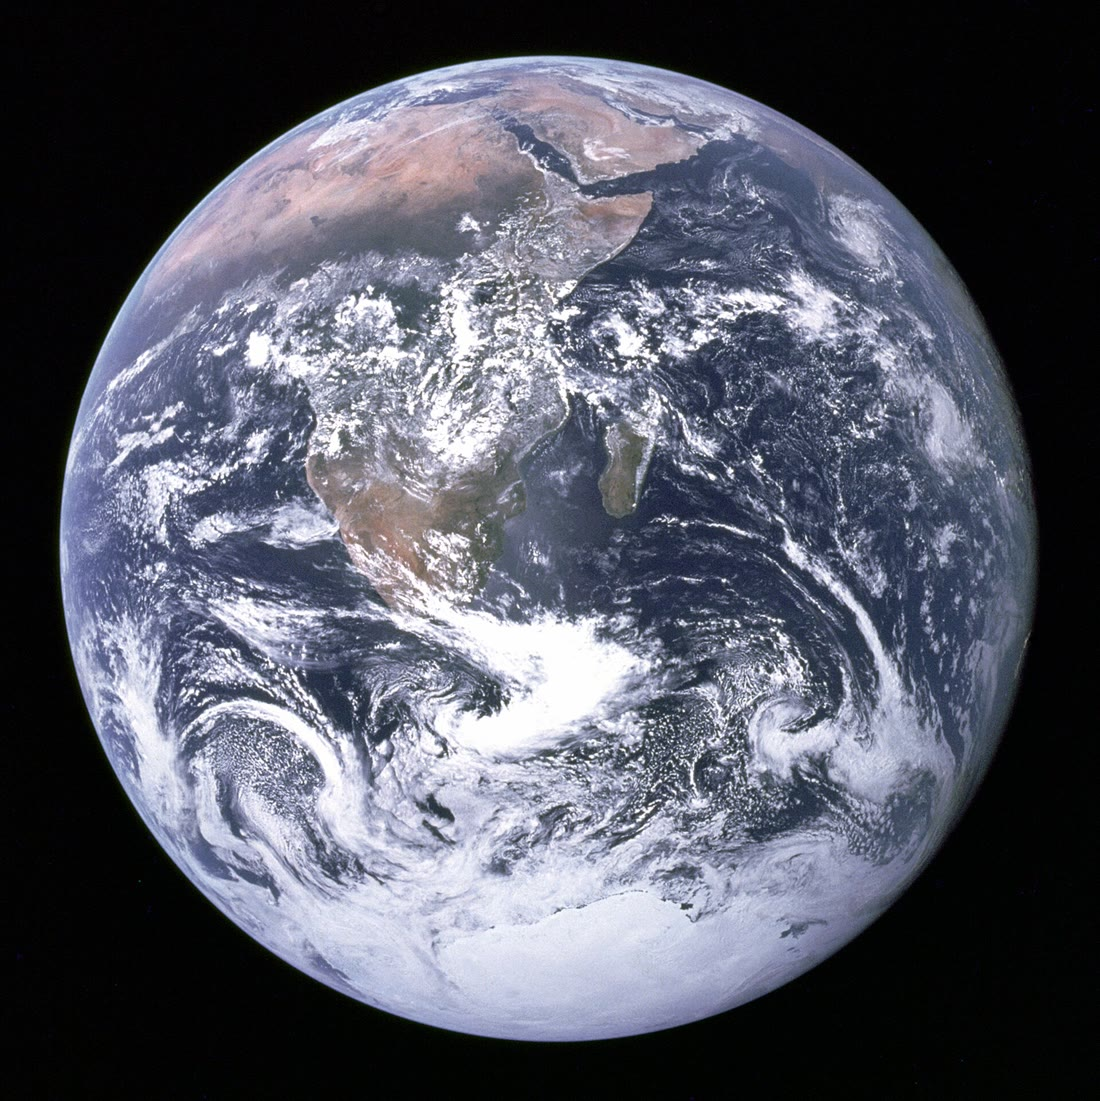
\includegraphics[width=0.5\linewidth]{images/book2/g10-nasa-apollo17-earth.jpg}

{\small La Tierra fotografiada por la tripulación del Apolo~17 camino de la
Luna, en diciembre de 1972: África, Arabia y el hielo de la Antártida.
Fotografía: NASA (dominio público).}
\end{omfigure}

\begin{recall}
Un lugar de la Tierra se localiza por su latitud, su ángulo al norte o al sur
del ecuador, y por su longitud, su ángulo al este o al oeste de un meridiano de
referencia; los meridianos unen los polos, y los paralelos rodean la Tierra
paralelos al ecuador (Libro 1). En un medio homogéneo la luz se propaga en
línea recta, y los rayos que llegan a la Tierra desde el lejanísimo Sol son
paralelos (los libros de física). En un triángulo rectángulo, el seno de un
ángulo agudo es el cateto opuesto dividido entre la hipotenusa, su coseno el
cateto contiguo dividido entre la hipotenusa, y su tangente el cateto opuesto
dividido entre el contiguo (los libros de matemáticas).
\end{recall}

\section{Una Tierra redonda}

Mucho antes de que nadie pudiera mirar la Tierra desde el espacio, varias
observaciones mostraban que es redonda.
\begin{itemize}
  \item \textbf{Barcos tras el horizonte.} Un barco que se aleja desaparece
        de abajo arriba, en cualquier dirección y en cualquier mar: la
        superficie del mar es curva en todas partes.
  \item \textbf{La sombra sobre la Luna.} Durante un eclipse de Luna, la
        sombra de la Tierra cae sobre la Luna. Su borde es siempre un arco de
        circunferencia, sea cual sea la hora de la noche; solo una esfera
        proyecta una sombra redonda en todas las direcciones.
  \item \textbf{Las estrellas cambian con la latitud.} Un viajero que va
        hacia el norte ve subir la estrella Polar sobre el horizonte, y las
        estrellas del cielo austral desaparecen por debajo de él: el
        horizonte del viajero se inclina a medida que avanza sobre una
        superficie curva.
  \item \textbf{La vuelta al mundo y la vista desde el espacio.} Barcos, y
        después aviones, han dado la vuelta al mundo en todas las
        direcciones; desde los años sesenta se ha fotografiado el planeta
        entero, redondo.
\end{itemize}

\begin{omfigure}
\begin{tikzpicture}[font=\small, >={Stealth[length=2.2mm]}]
  % sea surface: arc of a circle of radius 8 centred at (0,-8) (curvature exaggerated)
  \fill[omDef!10] plot[domain=-4.6:4.6, samples=60] (\x,{sqrt(64-\x*\x)-8}) -- (4.6,-2.2) -- (-4.6,-2.2) -- cycle;
  \draw[omDef!70!black, thick] plot[domain=-4.6:4.6, samples=60] (\x,{sqrt(64-\x*\x)-8});
  % observer on a small tower at x=-4 (surface y=-1.072), eye at y=-0.235
  \draw[black!70, line width=1pt] (-4,-1.072) -- (-4,-0.235);
  \fill (-4,-0.235) circle (2pt);
  \node[anchor=east, align=right] at (-4.1,-0.2) {ojo del\\observador};
  % line of sight tangent at x=-0.5 (y=-0.0156, slope 0.0626)
  \draw[omThm!80!black, thick] (-4,-0.235) -- (4.4,0.290);
  \node[omThm!80!black, anchor=south, rotate=3.6] at (1.3,0.1) {línea de visión};
  \fill[omThm!80!black] (-0.5,-0.0156) circle (1.4pt);
  % ship at x=3 (surface y=-0.584), tilted 22 degrees with the local vertical
  \begin{scope}[shift={(3,-0.584)}, rotate=-22]
    \fill[black!12] (-0.6,0) -- (0.6,0) -- (0.75,0.32) -- (-0.75,0.32) -- cycle;
    \draw[black!45, densely dashed] (-0.6,0) -- (0.6,0) -- (0.75,0.32) -- (-0.75,0.32) -- cycle;
    \draw[black!45, densely dashed] (0,0.32) -- (0,0.95);
    \draw[black!80, line width=1pt] (0,0.95) -- (0,1.55);
    \fill[black!80] (0,1.55) -- (0.32,1.25) -- (0,1.25) -- cycle;
  \end{scope}
  \node[anchor=north, align=center, font=\footnotesize] at (2.9,-1.25) {casco y parte baja del mástil\\ocultos por la curvatura};
  \node[anchor=north, font=\footnotesize] at (-0.5,-0.1) {horizonte};
\end{tikzpicture}

{\small Por qué un barco desaparece de abajo arriba: el observador solo ve lo
que queda por encima de la línea de visión que roza el mar en el horizonte.
La curvatura está muy exagerada.}
\end{omfigure}

\section{Eratóstenes mide la Tierra}

Eratóstenes de Cirene (276--194 a.\,C.) fue bibliotecario de Alejandría.
Había oído que en Siena, la actual Asuán, muy arriba en el Nilo, el Sol
iluminaba a mediodía todo el fondo de un pozo el día del solsticio de verano:
estaba entonces exactamente en el cenit. En Alejandría, en ese mismo momento,
un palo vertical proyectaba una sombra corta: los rayos del Sol formaban un
ángulo de unos \qty{7.2}{\degree} con la vertical, la cincuentava parte de
una vuelta completa.
% ledger: erat:method, erat:stadion

\begin{omfigure}
\begin{tikzpicture}[font=\small, >={Stealth[length=2.2mm]}]
  \def\R{2.4}
  \fill[omDef!8] (0,0) circle (\R);
  \draw[omDef!70!black, thick] (0,0) circle (\R);
  \coordinate (O) at (0,0);
  \coordinate (S) at (\R,0);
  \coordinate (A) at ({\R*cos(25)},{\R*sin(25)});
  \coordinate (T) at ({(\R+0.75)*cos(25)},{(\R+0.75)*sin(25)});
  \coordinate (T2) at ({(\R+1.75)*cos(25)},{(\R+1.75)*sin(25)});
  % radii
  \draw[black!70] (O) -- (S);
  \draw[black!70] (O) -- (A);
  \draw[black!40, densely dashed] (A) -- (T2);
  \fill (O) circle (1.5pt) node[below left] {centro};
  % stick at Alexandria, along the radius
  \draw[line width=1.6pt, black!85] (A) -- ($(A)!0.6!(T)$);
  % well at Syene
  \draw[black!80, thick] ({\R-0.38},-0.12) -- (\R,-0.12) ($(S)+(0,0.12)$) -- ({\R-0.38},0.12);
  % parallel sun rays coming from the right
  \foreach \y in {-1.6,-0.8,0.8,1.6} \draw[->, omThm!70, thick] (6.6,\y) -- (4.4,\y);
  \draw[->, omThm!85!black, thick] (6.6,0) -- (\R+0.05,0);
  \draw[->, omThm!85!black, thick] (6.6,{(\R+0.45)*sin(25)}) -- ({(\R+0.45)*cos(25)+0.03},{(\R+0.45)*sin(25)});
  \node[omThm!85!black, align=center, anchor=west] at (4.6,2.35) {luz del Sol:\\rayos paralelos};
  % angles
  \draw[omExo!80!black, thick] (0.75,0) arc (0:25:0.75);
  \node[omExo!80!black] at (1.05,0.22) {$\alpha$};
  \coordinate (Q) at ($(A)!0.6!(T)$);
  \draw[omExo!80!black, thick] ($(Q)+(0.8,0)$) arc (0:25:0.8);
  \node[omExo!80!black] at ($(Q)+({1.08*cos(12.5)},{1.08*sin(12.5)})$) {$\alpha$};
  \node[anchor=east] at ($(A)+(-0.12,0.18)$) {Alejandría};
  \node[anchor=north west] at ($(S)+(0.3,-0.12)$) {Siena};
  \node[font=\footnotesize, anchor=north] at ($(O)!0.5!(S)+(0.2,-0.05)$) {};
  \draw[<->, black!60] ({(\R-0.3)*cos(3)},{(\R-0.3)*sin(3)}) arc (3:22:{\R-0.3});
  \node[anchor=east, font=\footnotesize] at ({(\R-0.35)*cos(13)},{(\R-0.35)*sin(13)}) {$d$};
\end{tikzpicture}

{\small El razonamiento de Eratóstenes. En Siena el Sol está en el cenit: sus
rayos apuntan al centro de la Tierra. En Alejandría, un palo vertical, que
también apunta al centro, forma un ángulo $\alpha$ con los rayos. El ángulo
en el centro entre los dos lugares es el mismo $\alpha$. El ángulo está
exagerado: solo medía \qty{7.2}{\degree}.}
\end{omfigure}

\begin{proposition}[Relación de Eratóstenes]\label{prop:g10:measuring-the-earth:eratosthenes}
Si dos lugares están sobre el mismo meridiano, a una distancia $d$ uno de
otro, y a mediodía los rayos del Sol forman con la vertical ángulos que
difieren en $\alpha$ (en grados), la circunferencia de la Tierra es
\[
  C = \frac{\qty{360}{\degree}}{\alpha}\, d .
\]
\end{proposition}

\begin{proof}
El Sol está tan lejos que los rayos que llegan a los dos lugares son
paralelos. En cada lugar, la vertical apunta hacia el centro de la Tierra. En
la figura, el rayo que llega al palo y el radio que pasa por Siena son dos
rectas paralelas, y el radio que pasa por Alejandría corta a ambas: el ángulo
$\alpha$ entre el palo y el rayo y el ángulo en el centro entre los dos
radios son alternos internos, luego iguales. El arco $d$ es la misma fracción
de la circunferencia completa que el ángulo $\alpha$ de una vuelta entera:
$d/C = \alpha/\qty{360}{\degree}$.
\end{proof}

\begin{method}[Medir una circunferencia con dos sombras]\label{met:g10:measuring-the-earth:shadows}
\begin{enumerate}
  \item Elige dos lugares situados (casi) sobre el mismo meridiano y mide la
        distancia norte--sur $d$ entre ellos.
  \item A mediodía local del mismo día, mide en cada lugar el ángulo entre
        un palo vertical y los rayos del Sol: $\tan \theta = s/h$, donde $h$
        es la altura del palo y $s$ la longitud de su sombra. No mires nunca
        al Sol: el ángulo se lee solo en la sombra.
  \item Calcula la diferencia $\alpha$ entre los dos ángulos y aplica
        $C = (360/\alpha)\,d$.
\end{enumerate}
\end{method}

\begin{example}[Los números de Eratóstenes]\label{ex:g10:measuring-the-earth:numbers}
% ledger: erat:method, erat:stadion
Eratóstenes tomó como distancia de Alejandría a Siena 5000
\emph{estadios}, una unidad griega de longitud. Con $\alpha = 1/50$ de vuelta,
\[
  C = 50 \times 5000 = 250\,000 \text{ estadios}.
\]
¿Cuánto medía un estadio? Los historiadores todavía lo discuten. Con
\qty{157.2}{m}, $C \approx \qty{39300}{km}$; con \qty{166.7}{m},
$C \approx \qty{41700}{km}$. La circunferencia meridiana real es de
\qty{40008}{km}: en ambos casos, Eratóstenes acertó con un error de pocos
puntos porcentuales.
\end{example}

\begin{remark}[Lo que se supuso]\label{rem:g10:measuring-the-earth:assumptions}
Eratóstenes supuso una Tierra esférica, un Sol lo bastante lejano para que
sus rayos fueran paralelos, Siena exactamente sobre el trópico (donde el Sol
puede estar en el cenit) y Siena justo al sur de Alejandría. Todo ello era
casi cierto, pero no del todo: Asuán está unos \qty{3}{\degree} de longitud
al este de Alejandría. Lo que cuenta es la componente norte--sur de la
distancia, la que va a lo largo del meridiano.
% ledger: geonames:aswan, geonames:alexandria
\end{remark}

\section{La triangulación}

Medir una distancia larga sobre el terreno con una cadena o una regla es
lento, y a través de ríos, bosques y montañas, imposible. Los ángulos, en
cambio, se miden con gran precisión con un anteojo montado sobre un círculo
graduado, que se apunta por turnos a dos señales lejanas. A partir del
siglo XVIII, los topógrafos se valieron de ello para medir países enteros.

\begin{definition}[Geodesia]\label{def:g10:measuring-the-earth:geodesy}
La \emph{geodesia}\index{geodesia} es la ciencia que mide la forma y el
tamaño de la Tierra y la posición de los puntos de su superficie, y que
sigue cómo cambian con el tiempo.
\end{definition}

\begin{definition}[Triangulación]\label{def:g10:measuring-the-earth:triangulation}
La \emph{triangulación}\index{triangulacion@triangulación} localiza puntos
lejanos mediante una cadena de triángulos: un lado, la \emph{base}, se mide
sobre el terreno con gran cuidado; todos los ángulos de los triángulos se
miden desde sus vértices; todos los demás lados se calculan después.
\end{definition}

El cálculo se apoya en una relación entre los lados y los ángulos de
cualquier triángulo. En un triángulo $ABC$, se llama $a$, $b$, $c$ a los
lados opuestos a los vértices $A$, $B$, $C$, y también $A$, $B$, $C$ a los
ángulos en esos vértices.

\begin{proposition}[El teorema de los senos]\label{prop:g10:measuring-the-earth:sine-rule}
En todo triángulo $ABC$,
\[
  \frac{a}{\sin A} = \frac{b}{\sin B} = \frac{c}{\sin C}.
\]
\end{proposition}

\begin{proof}
Traza la altura desde $C$, que corta la recta $AB$ en $H$ (panel derecho de
la figura de abajo), y llama $h = CH$. En el triángulo rectángulo $AHC$,
$\sin A = h/b$, luego $h = b \sin A$. En el triángulo rectángulo $BHC$,
$\sin B = h/a$, luego $h = a \sin B$. Por tanto $b \sin A = a \sin B$, es
decir, $a/\sin A = b/\sin B$. (Si el ángulo en $B$ es obtuso, $H$ cae más
allá de $B$, y el ángulo del triángulo rectángulo en $B$ es
$\qty{180}{\degree} - B$, que tiene el mismo seno.) El mismo razonamiento
con la altura desde $A$ da $b/\sin B = c/\sin C$.
\end{proof}

\begin{omfigure}
\begin{tikzpicture}[font=\small, >={Stealth[length=2mm]}]
  \begin{scope}
    \coordinate (A) at (0,0); \coordinate (B) at (2.0,0.25);
    \coordinate (C) at (0.9,1.9); \coordinate (D) at (3.0,2.1);
    \coordinate (E) at (1.9,3.8); \coordinate (F) at (3.9,4.1);
    \coordinate (G) at (2.7,5.6);
    \draw[black!60] (A) -- (C) -- (B) (C) -- (D) -- (B) (C) -- (E) -- (D) -- (F) -- (E) -- (G) -- (F);
    \draw[omThm!85!black, line width=2pt] (A) -- (B);
    \foreach \p in {A,B,C,D,E,F,G} \fill (\p) circle (1.6pt);
    \node[below left] at (A) {$A$}; \node[below right] at (B) {$B$};
    \node[left] at (C) {$C$}; \node[right] at (D) {$D$};
    \node[left] at (E) {$E$}; \node[right] at (F) {$F$}; \node[above] at (G) {$G$};
    \node[omThm!85!black, anchor=north, font=\footnotesize] at (1.25,-0.3) {base medida};
    \draw[omExo!80!black] ($(A)!0.28!(B)$) arc[start angle=7, end angle=64.6, radius=0.56];
    \draw[omExo!80!black] ($(B)!0.3!(A)$) arc[start angle=187, end angle=123, radius=0.6];
    \draw[black!50, densely dashed] (-0.5,0) -- (-0.5,5.6);
    \draw[->, black!70] (-0.5,5.0) -- (-0.5,5.8) node[above] {N};
    \node[rotate=90, font=\footnotesize, black!60, anchor=south] at (-0.5,2.6) {meridiano};
  \end{scope}
  \begin{scope}[xshift=6.2cm, yshift=0.6cm]
    \coordinate (A) at (0,0); \coordinate (B) at (4,0); \coordinate (C) at (1.4,2.6);
    \coordinate (H) at (1.4,0);
    \draw[thick] (A) -- (B) -- (C) -- cycle;
    \draw[omDef!80!black, densely dashed] (C) -- (H);
    \draw[omDef!80!black] (1.4,0.22) -- (1.62,0.22) -- (1.62,0);
    \node[below left] at (A) {$A$}; \node[below right] at (B) {$B$};
    \node[above] at (C) {$C$}; \node[below] at (H) {$H$};
    \node[omDef!80!black, anchor=west] at (1.4,1.05) {$h$};
    \node[anchor=south east] at (0.7,1.3) {$b$};
    \node[anchor=south west] at (2.75,1.35) {$a$};
    \node[anchor=north] at (2.7,-0.02) {$c$};
    \draw[omExo!80!black] (0.5,0) arc (0:61.7:0.5);
    \draw[omExo!80!black] (3.45,0) arc (180:135:0.55);
  \end{scope}
\end{tikzpicture}

{\small Izquierda: una cadena de triángulos tendida a lo largo de un
meridiano a partir de una base medida $AB$; los arcos marcan dos de los
muchos ángulos medidos con el instrumento. Derecha: la altura $h$ desde $C$,
escrita de dos maneras, da el teorema de los senos.}
\end{omfigure}

\begin{method}[Calcular una cadena de triangulación]\label{met:g10:measuring-the-earth:chain}
\begin{enumerate}
  \item En el primer triángulo $ABC$ se miden la base $c = AB$ y los
        ángulos en $A$ y en $B$; el tercer ángulo es
        $C = \qty{180}{\degree} - A - B$ (y su medida sirve para comprobar
        las otras).
  \item El teorema de los senos da los otros dos lados:
        $b = AC = c \sin B / \sin C$ y $a = BC = c \sin A / \sin C$.
  \item Un lado calculado se convierte en el lado conocido del triángulo
        siguiente, y así sucesivamente a lo largo de la cadena.
  \item Por último, la componente norte--sur de cada lado se calcula con el
        coseno de su ángulo con el meridiano, y se suman las componentes.
\end{enumerate}
\end{method}

\begin{example}[Un triángulo]\label{ex:g10:measuring-the-earth:triangle}
Se mide una base $AB = \qty{8.000}{km}$; desde $A$, la señal $C$ se ve a
\qty{70}{\degree} de la dirección de $B$, y desde $B$, a
\qty{60}{\degree} de la dirección de $A$. Entonces $C = \qty{50}{\degree}$ y
\[
  AC = \frac{8.000 \times \sin 60^\circ}{\sin 50^\circ} = \frac{8.000 \times 0.8660}{0.7660}
  \approx \qty{9.044}{km}, \qquad
  BC = \frac{8.000 \times \sin 70^\circ}{\sin 50^\circ} \approx \qty{9.814}{km}.
\]
No se recorrió a pie ninguna distancia salvo la base.
\end{example}

\begin{example}[El meridiano del metro]\label{ex:g10:measuring-the-earth:meridian}
% ledger: metre:1791, metre:survey, geonames:dunkirk, geonames:barcelona (arc computed in figdata/grade-10/meridian_degree.py)
En marzo de 1791 se definió el metro como la diezmillonésima parte de la
distancia del polo al ecuador a lo largo de un meridiano. Para hallar esa
distancia, dos astrónomos, Jean-Baptiste Delambre y Pierre Méchain, midieron
por \omterm{def:g10:measuring-the-earth:triangulation}{triangulación} el arco de meridiano de Dunkerque, en el mar del Norte, a
Barcelona, en el Mediterráneo: casi siete años de trabajo, Delambre en los
dos tercios del norte y Méchain en el tercio del sur. Las dos ciudades
difieren en \qty{9.646}{\degree} de latitud; sobre el elipsoide moderno, el
arco entre sus paralelos mide \qty{1072.2}{km}. Conocer la longitud de un
arco y su diferencia de latitud da la longitud de un grado; la forma de la
Tierra da después el cuarto de meridiano entero. En 1799 se fabricaron
patrones de platino del nuevo metro, que se guardaron en los Archivos
nacionales.
\end{example}

\begin{history}[El círculo repetidor]
Los ángulos del meridiano del metro se midieron con un \emph{círculo
repetidor}, un instrumento construido por Jean-Charles de Borda: dos
anteojos sobre un círculo graduado, apuntados alternativamente a dos señales
muchas veces seguidas, de modo que los errores de lectura de la graduación
quedan divididos por el número de repeticiones.
\begin{center}
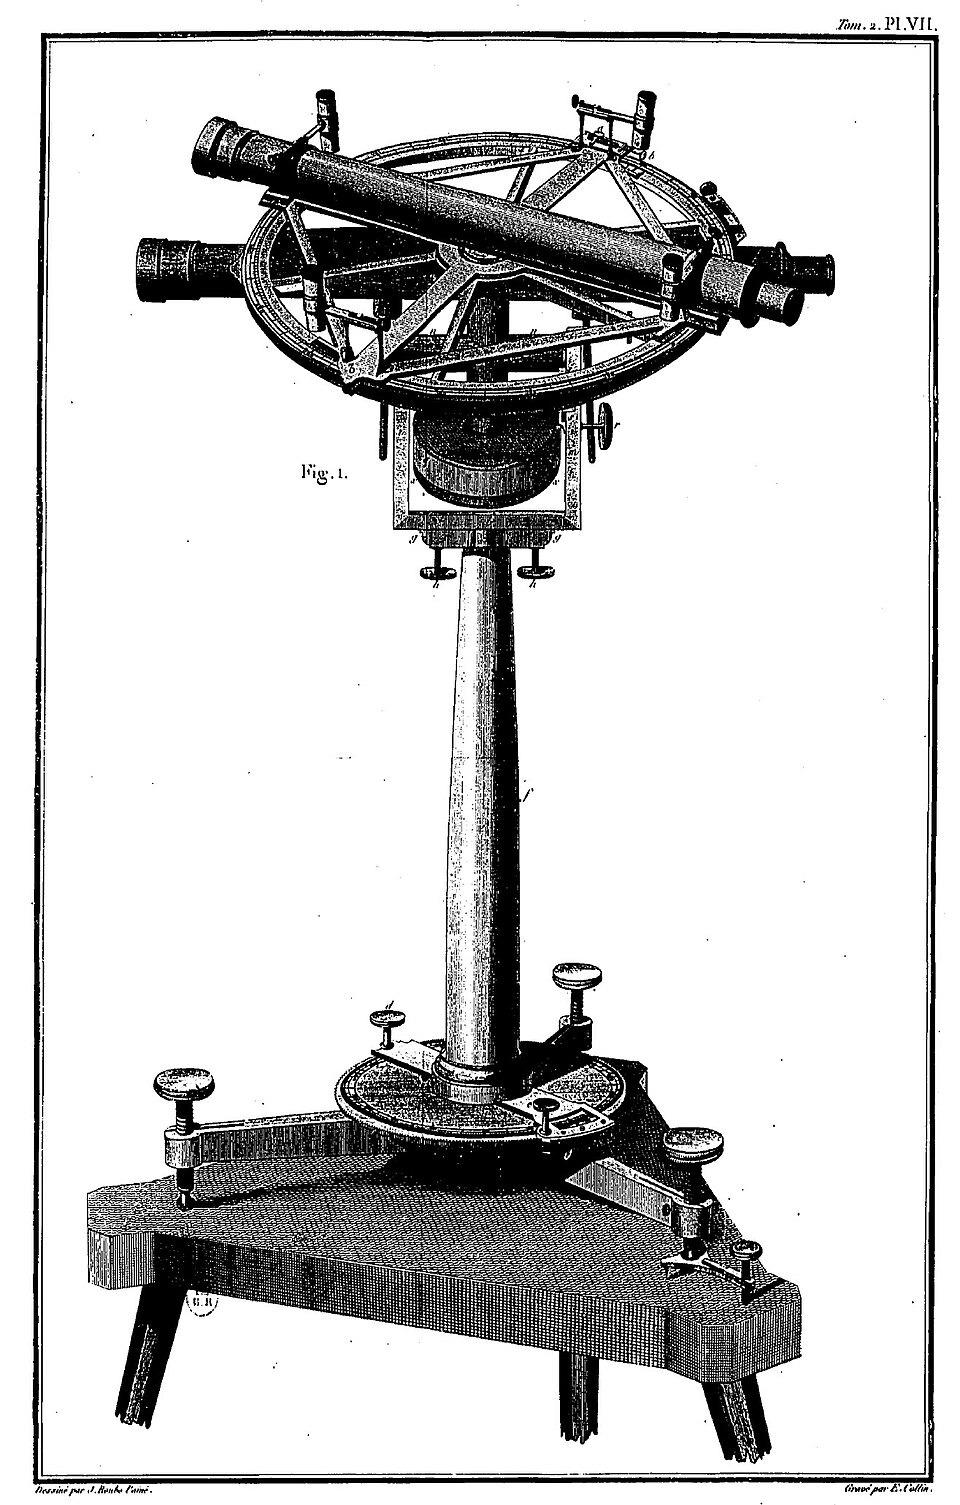
\includegraphics[width=0.3\linewidth]{images/book2/g10-delambre-repeating-circle.jpg}

{\small Un círculo repetidor montado para medir ángulos horizontales, tal
como aparece grabado en el relato de la medición de Delambre (1807). Dominio
público (Wikimedia Commons).}
\end{center}
\end{history}

\section{Una Tierra achatada}

Hacia 1687, Isaac Newton dedujo de su teoría de la gravitación que una
Tierra en rotación tiene que ser un esferoide achatado por los polos y
abultado en el ecuador. Las medidas de grados de meridiano realizadas por
los astrónomos del Observatorio de París parecían decir lo contrario: una
Tierra alargada hacia los polos. La cuestión se zanjó midiendo la longitud de
un grado de latitud en lugares lo más alejados posible.
% ledger: figure:expeditions

\begin{omfigure}
\begin{tikzpicture}[font=\small, >={Stealth[length=2mm]}]
  \def\a{3.0} \def\b{2.3}
  \draw[black!35, densely dashed] (0,0) circle (\a);
  \fill[omDef!8] (0,0) ellipse ({\a} and {\b});
  \draw[omDef!70!black, thick] (0,0) ellipse ({\a} and {\b});
  \draw[black!50] (-3.4,0) -- (3.7,0);
  \draw[black!50] (0,-2.6) -- (0,3.3);
  \draw[<->, omThm!85!black] (0,-0.3) -- (\a,-0.3);
  \node[omThm!85!black, below] at (1.5,-0.3) {$a$};
  \draw[<->, omThm!85!black] (-0.3,0) -- (-0.3,\b);
  \node[omThm!85!black, left] at (-0.3,1.15) {$b$};
  \node[above right] at (0,\b) {N};
  \node[anchor=south east] at (3.0,-2.5) {};
  \node[anchor=west] at (3.7,0) {ecuador};
  % normal at t = 45 deg: P = (2.121, 1.626); crosses the equator at (0.874,0), the axis at (0,-1.14)
  \coordinate (P) at (2.121,1.626);
  \draw[omExo!85!black, thick] (P) -- ($(P)!1.35!(0.874,0)$);
  \draw[omExo!85!black, thick, ->] (P) -- ($(P)!-0.45!(0.874,0)$);
  \fill (P) circle (1.6pt);
  \node[anchor=west, align=left, font=\footnotesize] at (2.85,2.35) {vertical del lugar\\(plomada)};
  \draw[omExo!85!black] (1.45,0) arc (0:52.5:0.58);
  \node[omExo!85!black] at (1.62,0.32) {$\varphi$};
  \fill (0,0) circle (1.3pt);
  \node[anchor=north east, font=\footnotesize] at (0,0) {centro};
  \node[black!50, font=\footnotesize, anchor=south] at (-2.2,2.15) {esfera};
\end{tikzpicture}

{\small Una Tierra achatada, con el \omterm{def:g10:measuring-the-earth:ellipsoid}{achatamiento} muy exagerado (el real es
demasiado pequeño para verse a esta escala). La vertical de un lugar es
perpendicular a la superficie; no apunta exactamente al centro. La latitud
$\varphi$ del lugar es el ángulo entre su vertical y el plano del ecuador.}
\end{omfigure}

La latitud se mide con las estrellas: es el ángulo entre la vertical del
lugar y el plano del ecuador. En una Tierra achatada, la superficie está
menos curvada cerca de los polos que cerca del ecuador. Donde la superficie
está menos curvada, hay que recorrer más camino sobre ella para que la
vertical gire un grado: \emph{un grado de latitud es más largo cerca de los
polos}.

\begin{history}[Laponia y Perú]
% ledger: figure:expeditions, figure:degrees
En 1735, la Academia de Ciencias de París envió una expedición al ecuador,
a la provincia española del Perú (hoy Ecuador), que trabajó allí nueve años,
hasta 1744. En 1736--1737, una segunda expedición, dirigida por Pierre-Louis
Moreau de Maupertuis con el joven matemático Alexis Clairaut, midió un grado
de meridiano en Laponia, cerca del círculo polar ártico. El grado de Laponia
dio 57\,437 \emph{toesas} (la antigua unidad de longitud; unos
\qty{111.95}{km}), y el de Perú solo 56\,737 toesas: el grado es más largo
cerca del polo, y Newton tenía razón. Los dos números implicaban un
\omterm{def:g10:measuring-the-earth:ellipsoid}{achatamiento} de alrededor de $1/205$ ---demasiado grande, como mostraron
mediciones posteriores---, pero la cuestión del signo quedó resuelta.
\end{history}

\begin{omfigure}
\begin{tikzpicture}
\begin{axis}[omrecord, width=0.82\linewidth, height=5.4cm, xmin=0, xmax=90,
  ymin=110.45, ymax=111.8, xlabel={latitud (\unit{\degree})},
  ylabel={longitud de \qty{1}{\degree} de latitud (km)}, xtick={0,15,...,90},
  ytick={110.6,110.8,...,111.8}, yticklabel style={/pgf/number format/fixed, /pgf/number format/fixed zerofill, /pgf/number format/precision=1}]
\addplot[omDef!85!black, line width=1.1pt] table[x=lat_deg, y=deg_km] {figdata/out/grade-10-meridian_degree.dat};
\addplot[only marks, mark=*, mark size=1.8pt, omThm!85!black] coordinates {(0,110.574) (45,111.132) (66,111.507) (90,111.694)};
\node[anchor=south west, font=\footnotesize] at (axis cs:2,110.6) {110.57 km};
\node[anchor=north east, font=\footnotesize] at (axis cs:89,111.56) {111.69 km};
\node[anchor=north west, font=\footnotesize] at (axis cs:46,111.12) {111.13 km};
\node[anchor=south east, font=\footnotesize] at (axis cs:65,111.53) {111.51 km a \ang{66} (Laponia)};
\end{axis}
\end{tikzpicture}

{\small Longitud de un grado de latitud sobre el \omterm{def:g10:measuring-the-earth:ellipsoid}{elipsoide de referencia} de
la \cref{def:g10:measuring-the-earth:ellipsoid}, del ecuador al polo.
Calculada a partir del elipsoide WGS~84.}
\end{omfigure}

\begin{definition}[Elipsoide de referencia y achatamiento]\label{def:g10:measuring-the-earth:ellipsoid}
Un \emph{elipsoide de referencia}\index{elipsoide de referencia} es la
superficie que se obtiene al hacer girar una elipse alrededor de su eje
corto, elegida para ajustarse lo mejor posible a la forma de la Tierra. Su
\emph{radio ecuatorial} es $a$, su \emph{radio polar} $b$, y su
\emph{achatamiento}\index{achatamiento} es
\[
  f = \frac{a-b}{a}.
\]
\end{definition}

\begin{proposition}[Las dimensiones de la Tierra]\label{prop:g10:measuring-the-earth:dimensions}
% ledger: wgs84:ellipsoid, earth:Req, earth:Rpol, earth:Rmean (lengths computed in figdata/grade-10/meridian_degree.py)
El \omterm{def:g10:measuring-the-earth:ellipsoid}{elipsoide de referencia} que usa el posicionamiento por satélite (WGS~84) tiene
\[
  a = \qty{6378.137}{km}, \qquad b = \qty{6356.752}{km}, \qquad
  f = \frac{1}{298.257}.
\]
El radio polar es \qty{21.4}{km} más corto que el radio ecuatorial. El
ecuador mide \qty{40075}{km} y un meridiano, de polo a polo y vuelta,
\qty{40008}{km}; el cuarto de meridiano, del ecuador a un polo, mide
\qty{10001.966}{km}. Un grado de latitud mide \qty{110.574}{km} en el
ecuador y \qty{111.694}{km} en los polos. Un grado de longitud mide
\qty{111.32}{km} sobre el ecuador y se acorta hacia los polos
aproximadamente como $\cos \varphi$.
\end{proposition}

\begin{example}[Un grado de longitud]\label{ex:g10:measuring-the-earth:longitude}
Un paralelo de latitud $\varphi$ es una circunferencia cuyo radio es la
distancia al eje, aproximadamente $R \cos \varphi$. A \qty{60}{\degree} N,
su longitud es más o menos la mitad de la del ecuador, y un grado de
longitud mide unos $111.32 \times \cos 60^\circ \approx \qty{55.7}{km}$ (el
elipsoide da \qty{55.80}{km}).
\end{example}

\begin{remark}[¿Hasta qué punto es redonda?]\label{rem:g10:measuring-the-earth:round}
Un \omterm{def:g10:measuring-the-earth:ellipsoid}{achatamiento} de $1/298$ es pequeño. En un globo de \qty{30}{cm} de
diámetro, el diámetro polar solo sería \qty{1}{mm} más corto que el
ecuatorial: invisible. La fosa oceánica más profunda, a casi \qty{11}{km}
bajo el nivel del mar, sería un arañazo de apenas un cuarto de milímetro de
profundidad. Para la mayoría de los usos, la Tierra es una esfera de radio
medio \qty{6371}{km}; para posiciones precisas, hace falta el elipsoide.
% ledger: earth:Rmean, usgs:trench-depth
\end{remark}

\section{La geodesia hoy}

\begin{omfigure}
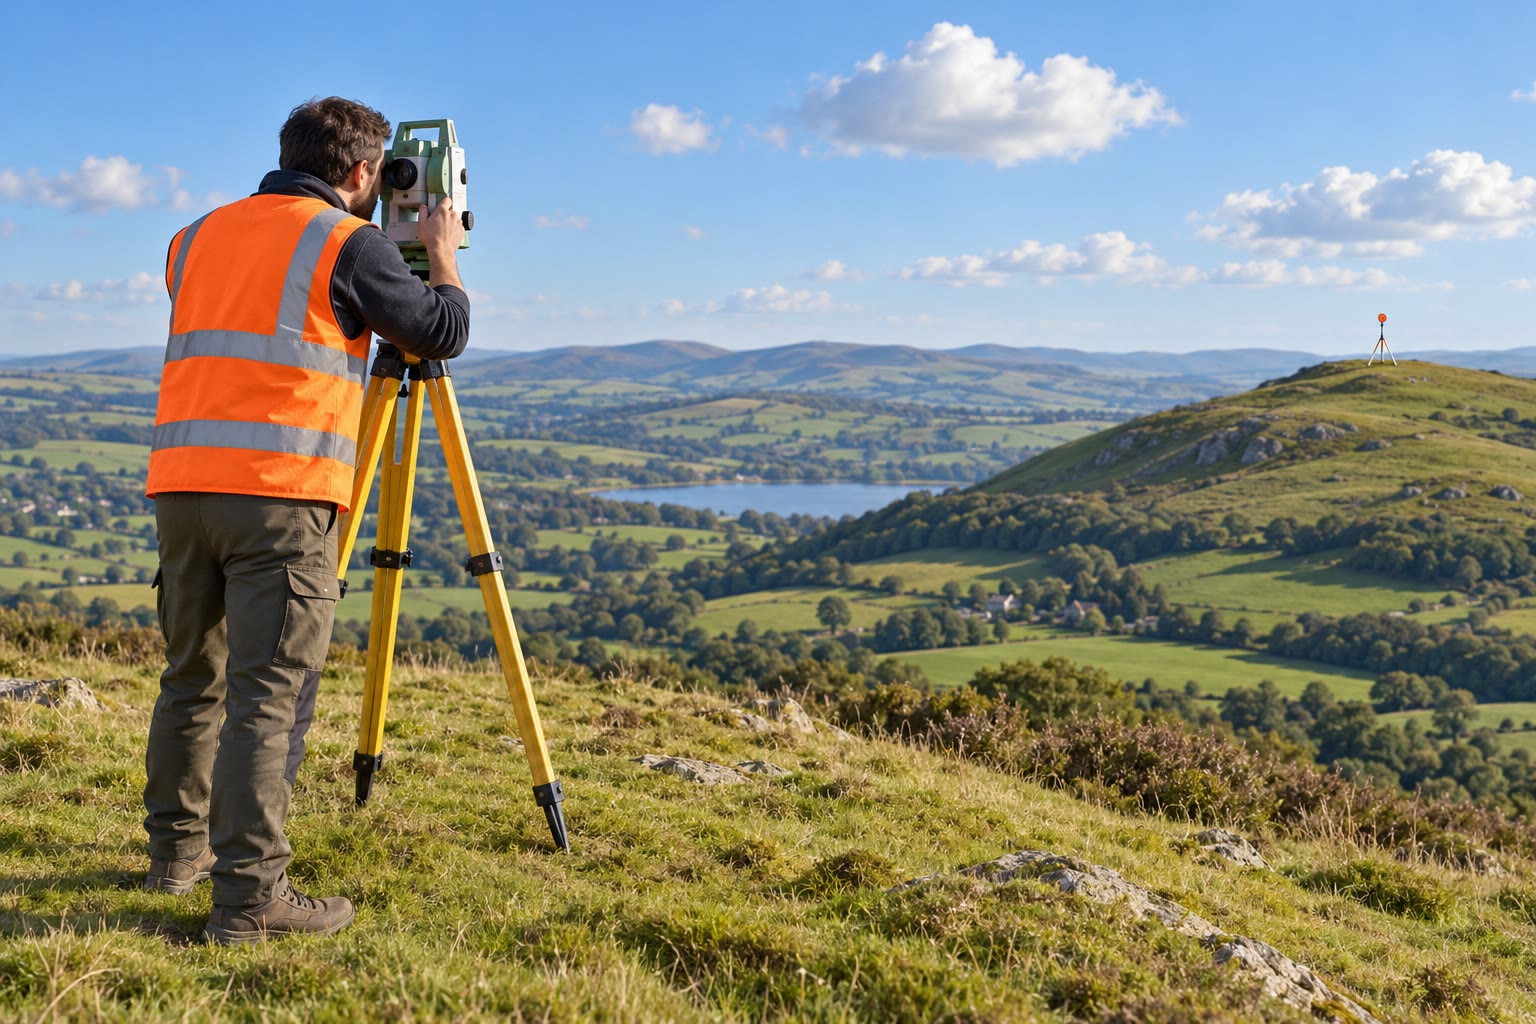
\includegraphics[width=0.7\linewidth]{images/book2/ai/g10-surveyor-theodolite.jpg}

{\small Un topógrafo trabajando con un instrumento moderno que mide ángulos
y, con un haz de luz, distancias; en la colina del fondo se alza una señal
geodésica.}
\end{omfigure}

Las grandes triangulaciones de los siglos XVIII y XIX han sido sustituidas
por los satélites. Un receptor en el suelo capta las señales de varios
satélites cuyas posiciones se conocen en cada instante, y calcula su propia
posición a partir de los tiempos de viaje de las señales (Libro 1). Redes de
receptores permanentes, fijados a la roca de todo el mundo, miden sus
posiciones sin interrupción. Definen el marco de referencia en el que se da
cada mapa y cada posición por satélite, y se mueven: muestran cómo las
placas de la litosfera derivan unos pocos centímetros al año
(\cref{ch:g11:plate-motions}).
% ledger: usgs:gps

\begin{inthefield}[Medir el terreno hoy]
Los geodestas anclan antenas sobre pilares de hormigón asentados en la roca,
lejos de edificios y árboles, y registran sus posiciones cada pocos segundos
durante años. Las combinan con medidas de radiotelescopios que observan
galaxias muy lejanas y con haces láser disparados hacia satélites que llevan
espejos. Los topógrafos de las obras y del campo siguen midiendo ángulos y
distancias con instrumentos sobre trípodes, y los enlazan con el marco de
los satélites.
\end{inthefield}

\section{Ejercicios}

\begin{exercise}[$\star$]\label{exo:g10:measuring-the-earth:1}
Da tres observaciones, posibles sin despegarse del suelo, que muestren que
la Tierra es redonda. Para cada una, explica en una frase por qué una
Tierra plana no podría producirla.
\end{exercise}

\begin{exercise}[$\star$]\label{exo:g10:measuring-the-earth:2}
¿Qué es la \omterm{def:g10:measuring-the-earth:geodesy}{geodesia}? ¿Qué es la \omterm{def:g10:measuring-the-earth:triangulation}{triangulación}, y qué única longitud hay que
medir sobre el terreno en una \omterm{def:g10:measuring-the-earth:triangulation}{triangulación}?
\end{exercise}

\begin{exercise}[$\star$]\label{exo:g10:measuring-the-earth:3}
Eratóstenes halló que el ángulo entre los rayos del Sol y la vertical en
Alejandría era $1/50$ de vuelta completa cuando el Sol estaba en el cenit en
Siena, a 5000 estadios. Calcula la circunferencia en estadios y después en
kilómetros, tomando un estadio de \qty{157.2}{m}.
\end{exercise}

\begin{exercise}[$\star$]\label{exo:g10:measuring-the-earth:4}
Un grado de latitud mide unos \qty{111}{km}. ¿Cuánto mide un minuto de
latitud ($1/60$ de grado)? ¿Cuánto mide, aproximadamente, el meridiano del
ecuador al polo?
\end{exercise}

\begin{exercise}[$\star$]\label{exo:g10:measuring-the-earth:5}
Con el radio ecuatorial \qty{6378.137}{km} y el radio polar
\qty{6356.752}{km}, calcula la diferencia entre los dos radios y el
\omterm{def:g10:measuring-the-earth:ellipsoid}{achatamiento} $f = (a-b)/a$. Expresa $f$ como uno dividido entre un número
entero.
\end{exercise}

\begin{exercise}[$\star\star$]\label{exo:g10:measuring-the-earth:6}
Dos ciudades están sobre el mismo meridiano, a \qty{500}{km} una de otra. A
mediodía del mismo día, un palo vertical de \qty{1.00}{m} de altura proyecta
una sombra de \qty{0.364}{m} en la ciudad del sur y de \qty{0.456}{m} en la
del norte. Calcula el ángulo entre los rayos del Sol y la vertical en cada
ciudad y, después, la circunferencia de la Tierra.
\end{exercise}

\begin{exercise}[$\star\star$]\label{exo:g10:measuring-the-earth:7}
En un triángulo $ABC$, la base $AB = \qty{10.00}{km}$, el ángulo en $A$ mide
\qty{62}{\degree} y el ángulo en $B$ mide \qty{71}{\degree}. Calcula el
ángulo en $C$ y las longitudes $AC$ y $BC$.
\end{exercise}

\begin{exercise}[$\star\star$]\label{exo:g10:measuring-the-earth:8}
Un avión vuela hacia el oeste a lo largo del paralelo \qty{60}{\degree} N,
desde la longitud \qty{10}{\degree} E hasta la longitud \qty{20}{\degree} O.
Con un grado de longitud de $111.3 \cos \varphi$ km, calcula la distancia
que recorre. ¿Cuánto mediría el mismo cambio de longitud sobre el ecuador?
\end{exercise}

\begin{exercise}[$\star\star$]\label{exo:g10:measuring-the-earth:9}
El ojo de un observador está a $h = \qty{2}{m}$ sobre un mar en calma. La
visual hacia el horizonte roza el mar en $T$; el centro de la Tierra es $O$
y el ojo, $E$. Explica por qué el triángulo $OTE$ tiene un ángulo recto en
$T$ y usa después el teorema de Pitágoras con $R = \qty{6371}{km}$ para
demostrar que la distancia al horizonte es de aproximadamente $\sqrt{2Rh}$;
calcúlala.
\end{exercise}

\begin{exercise}[$\star\star$]\label{exo:g10:measuring-the-earth:10}
Lee la curva de las longitudes de un grado. ¿Entre qué latitudes cambia más
deprisa la longitud de un grado? Explica en dos frases por qué un grado de
latitud es más largo cerca de los polos que cerca del ecuador.
\end{exercise}

\begin{exercise}[$\star\star$]\label{exo:g10:measuring-the-earth:11}
El arco de meridiano de Dunkerque a Barcelona abarca \qty{9.646}{\degree}
de latitud y mide \qty{1072.2}{km}. Calcula la longitud media de un grado a
lo largo de él. Si todos los grados tuvieran esa longitud, ¿cuánto mediría
el cuarto de meridiano? Compáralo con \qty{10002.0}{km} y explica la pequeña
diferencia.
\end{exercise}

\begin{exercise}[$\star\star\star$]\label{exo:g10:measuring-the-earth:12}
Eratóstenes midió un ángulo de \qty{7.2}{\degree} y una distancia de 5000
estadios. Si su ángulo hubiera tenido un error de \qty{0.1}{\degree} (por
defecto), ¿en qué porcentaje se habría equivocado su circunferencia, y en
qué sentido? ¿Cuál de sus dos medidas crees que era la menos precisa?
\end{exercise}

\begin{exercise}[$\star\star\star$]\label{exo:g10:measuring-the-earth:13}
Una cadena de dos triángulos: en $ABC$, $AB = \qty{6.000}{km}$,
$A = \qty{55}{\degree}$, $B = \qty{75}{\degree}$. En el triángulo siguiente,
$ACD$, construido sobre el lado $AC$, el ángulo en $A$ mide
\qty{50}{\degree} y el ángulo en $C$, \qty{68}{\degree}. Calcula $AC$ y
después $AD$.
\end{exercise}

\begin{exercise}[$\star\star\star$]\label{exo:g10:measuring-the-earth:14}
¿A qué latitud mide un grado de longitud la mitad que sobre el ecuador? ¿A
qué latitud mide la décima parte? Explica por qué ninguna de las dos
respuestas depende del tamaño de la Tierra.
\end{exercise}

\begin{exercise}[$\star\star\star$]\label{exo:g10:measuring-the-earth:15}
Usa los valores del elipsoide: un grado de latitud mide \qty{110.574}{km} en
el ecuador y \qty{111.694}{km} en el polo. Sobre una esfera del mismo radio
medio, un grado mediría \qty{111.195}{km} en todas partes. ¿En cuántos
metros se equivocaría un topógrafo que supusiera una esfera en un grado en
el ecuador, y en un grado en el polo? ¿Por qué un mapa que da posiciones al
metro tiene que calcularse sobre el elipsoide?
\end{exercise}

\section{Problema: el metro y el meridiano}

\begin{problem}[{Problema de fin de semana --- de la sombra de Eratóstenes a
la longitud del primer metro}]
\label{pb:g10:measuring-the-earth:1}
% ledger: geonames:aswan, geonames:alexandria, erat:method, metre:1791, metre:survey, wgs84:ellipsoid (arc lengths and degree lengths computed in figdata/grade-10/meridian_degree.py)
Un estudiante reconstruye la historia de la medición de la Tierra con
números modernos. Asuán, la antigua Siena, está a la latitud
\qty{24.09}{\degree} N y Alejandría a \qty{31.20}{\degree} N; sobre el
elipsoide moderno, el arco de meridiano entre sus dos paralelos mide
\qty{788}{km}. Sobre el elipsoide, un grado de latitud mide
\qty{110.57}{km} en el ecuador, \qty{111.13}{km} a \qty{45}{\degree} y
\qty{111.51}{km} a \qty{66}{\degree}, y el cuarto de meridiano mide
\qty{10001.966}{km}.

\medskip
\noindent\textbf{Parte I --- Otra vez Eratóstenes.}
\begin{enumerate}
  \item Calcula la diferencia de latitud entre Asuán y Alejandría.
  \item ¿Qué fracción de una vuelta completa representa? Compárala con el
        $1/50$ de Eratóstenes.
  \item Calcula la circunferencia de la Tierra que da el método de
        Eratóstenes con estos números modernos.
  \item Las dos ciudades no están sobre el mismo meridiano: Asuán está unos
        \qty{3}{\degree} de longitud al este de Alejandría. ¿Qué distancia
        hay que usar en el método: la distancia en línea recta entre las
        ciudades o el arco de meridiano entre sus paralelos? ¿Por qué?
  \item ¿Por qué hay que medir las dos sombras el mismo día, a mediodía
        local?
\end{enumerate}

\medskip
\noindent\textbf{Parte II --- Una pequeña triangulación.}
Se mide una base $AB = \qty{12.000}{km}$. Desde $A$, la señal $C$ se ve a
\qty{58}{\degree} de $B$; desde $B$, a \qty{66}{\degree} de $A$. En el
triángulo siguiente, $ACD$, el ángulo en $A$ mide \qty{47}{\degree} y el
ángulo en $C$, \qty{75}{\degree}. El lado $AD$ apunta \qty{8}{\degree} al
este del norte.
\begin{enumerate}[resume]
  \item Calcula el ángulo en $C$ del triángulo $ABC$.
  \item Calcula el lado $AC$.
  \item Calcula el lado $BC$.
  \item Calcula el ángulo en $D$ del triángulo $ACD$ y después el lado $AD$.
  \item Calcula la distancia norte--sur entre $A$ y $D$.
  \item Con la longitud del grado a \qty{45}{\degree}, calcula la diferencia
        de latitud entre $A$ y $D$, en grados y en minutos de arco.
\end{enumerate}

\medskip
\noindent\textbf{Parte III --- Una Tierra achatada.}
\begin{enumerate}[resume]
  \item ¿En cuántos metros es más largo un grado de latitud a
        \qty{66}{\degree} que uno en el ecuador?
  \item Explica qué muestra esta diferencia sobre la forma de la Tierra.
  \item Sobre el elipsoide, $a = \qty{6378.137}{km}$ y
        $b = \qty{6356.752}{km}$. Calcula $a - b$ y el \omterm{def:g10:measuring-the-earth:ellipsoid}{achatamiento}.
  \item Explica por qué, en una Tierra achatada, la plomada en un lugar de
        latitud \qty{45}{\degree} no apunta exactamente al centro de la
        Tierra.
\end{enumerate}

\medskip
\noindent\textbf{Parte IV --- El primer metro.}
\begin{enumerate}[resume]
  \item Según la definición de 1791, ¿cuánto debería medir el cuarto de
        meridiano, en metros?
  \item El metro de platino de 1799 se fabricó a partir de un valor medido
        del meridiano. Si el cuarto de meridiano mide en realidad
        \qty{10001.966}{km}, ¿cuánto mide su diezmillonésima parte?
  \item ¿Era el metro de 1799 demasiado largo o demasiado corto respecto a
        su propia definición? ¿En qué fracción?
  \item La barra de platino copiaba fielmente la longitud calculada en la
        década de 1790. ¿Era el cuarto de meridiano calculado entonces
        demasiado largo o demasiado corto? Explícalo.
  \item ¿En cuántos milímetros era el primer metro más corto que la
        diezmillonésima parte del verdadero cuarto de meridiano? Compáralo con
        el grosor de una hoja de papel, unos \qty{0.1}{mm}.
\end{enumerate}
\end{problem}
